\subsection{Introduction}
\label{sec:kpimm:introduction}

The decay \BdToKpimm is a flavour-changing neutral-current process that, in the Standard Model (SM), proceeds through electroweak penguin or box diagrams.  In extensions to the SM, new heavy particles can enter the loop and modify observables such as branching fractions and angular distributions.

The previous angular analyses of \BdToKpimm performed by the \lhcb collaboration~\cite{kstmm-0.3fb,kstmm-1fb,kstmm-1fb-pprime,kstmm-3fb} have focused on the $796<\mkpi<996\mevcc$ region where the \kpi comes predominately from the P-wave decay $\decay{\Kstar(892)^{0}}{\kpi}$. 
A global analysis of the \CP-averaged angular observables measured using the \lhcb Run 1 data sample indicated differences with the presently-available SM predictions at the level of 3.4 standard deviations~\cite{kstmm-3fb}. The results of the measurement of the observable $P_{5}^{'}$, which exhibits a local deviation from the SM predictions, is shown in Fig.~\ref{fig:kpimm:p5prime}.

\begin{figure}[!b]
\centering
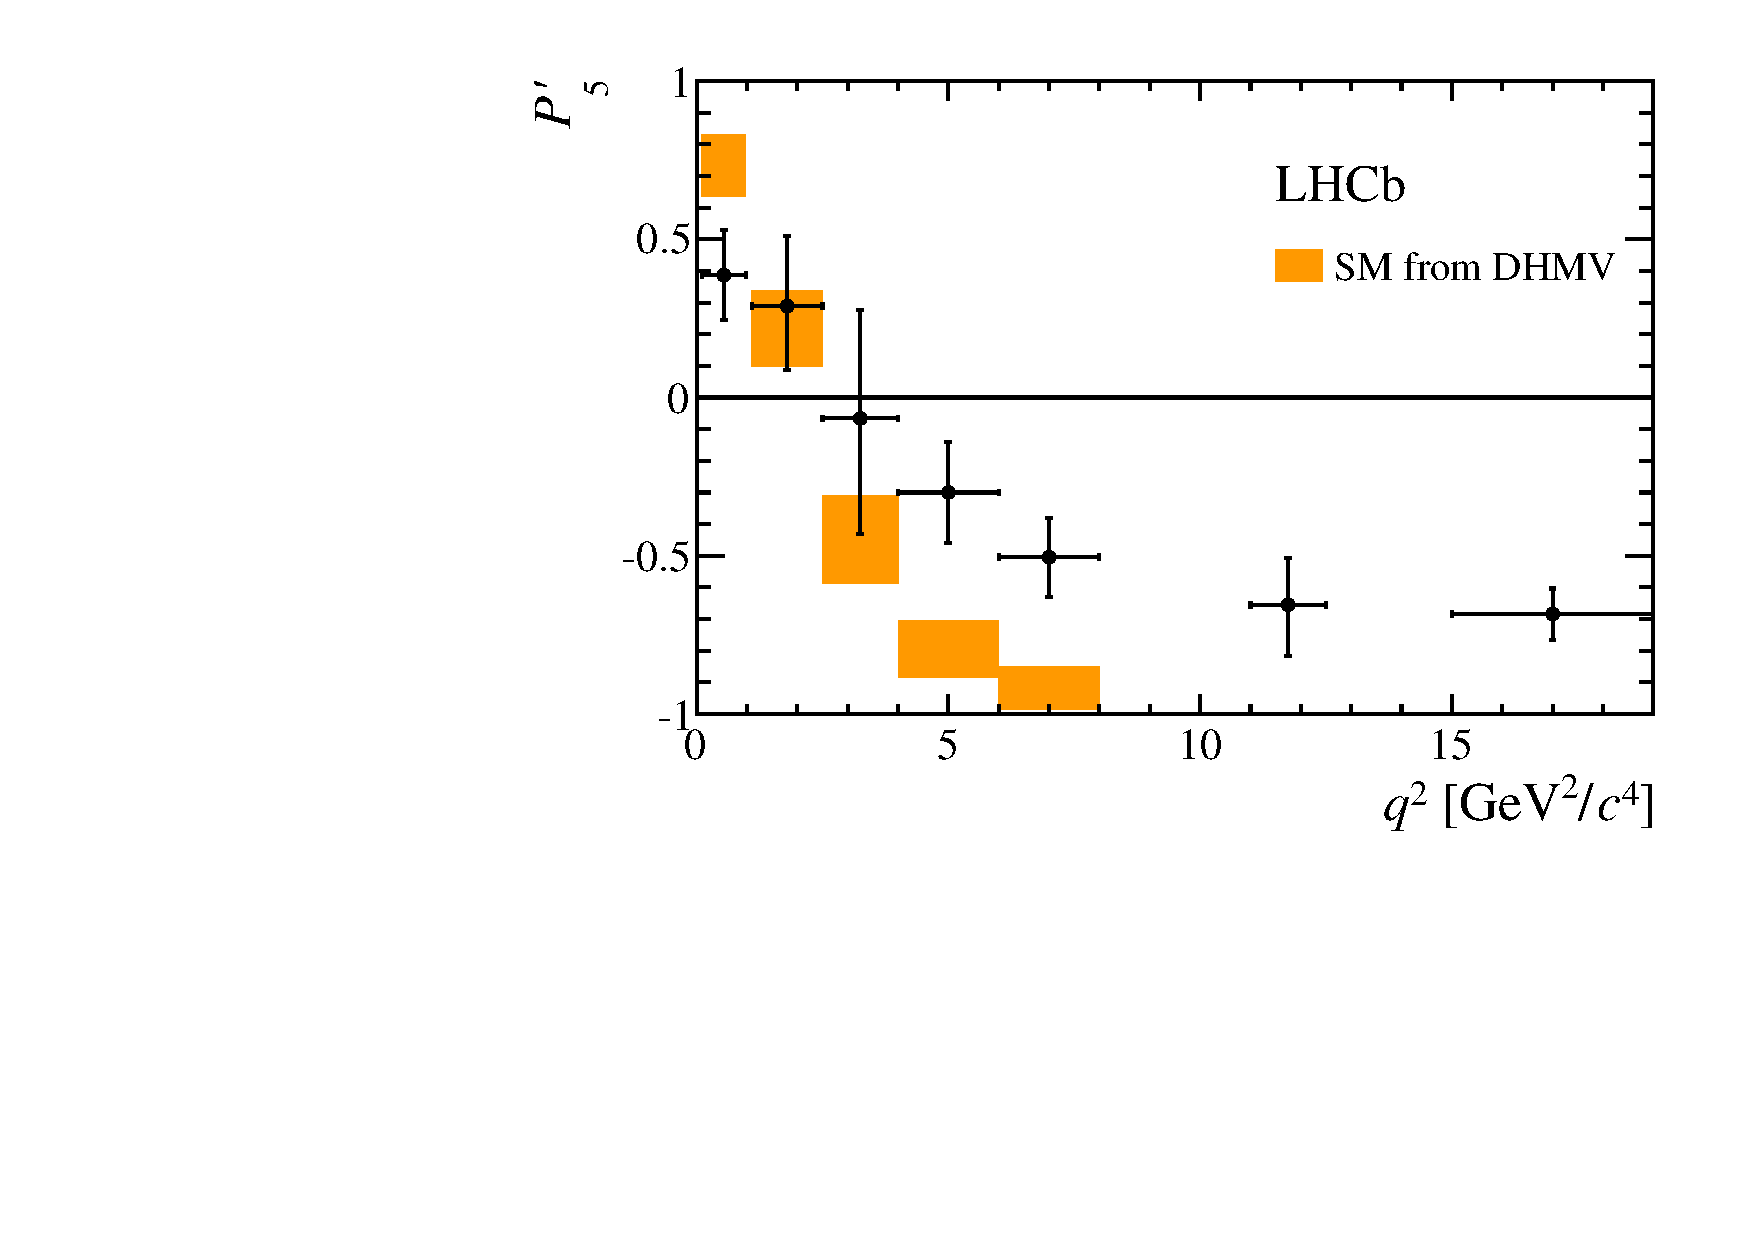
\includegraphics[width=0.8\textwidth]{figs/kpimm/introduction/P5prime.pdf}
\caption{Results of the measurement of the observable $P_{5}^{'}$ by the \lhcb collaboration. The SM predictions are taken from Ref.~\cite{pprime-theory}.}
\label{fig:kpimm:p5prime}
\end{figure}

This set of measurements is widely discussed in the literature (see for instance \cite{DescotesGenon:2013wba,Beaujean:2013soa,Crivellin:2015mga,Lyon:2014hpa} and references therein). It is presently still not clear if this discrepancy is caused by New Physics or by unaccounted hadronic effects. 
Since short distance effects are universal and should appear coherently in all $b\to s \mu\mu$ transitions, measuring other $b\to s\mu\mu$ transitions can help to shed light on this situation. Recently, the S-wave contribution to \BdToKpimm decays has been measured in the $644<\mkpi<1200\mevcc$ region~\cite{s-wave}. 

\begin{table}[!tb]
\caption{The expected resonant contributions with different spin-parity, $J^P$, above the \KstP mass range (adapted from Ref.~\cite{lu-wang}).}
\label{tab:introduction:states}
\centering
\begin{tabular}{c|c|c|c|r}
    Resonance & $J^{P}$ & Mass (\mevcc) & Full width (\mevcc)  & $\mathcal{B}(K\pi)~(\%)$ \\
   \hline
   $K^\ast(1410)^0$ & $1^{-}$& $1414 \pm 15$& $232 \pm 21$  & 6.6 $\pm$ 1.3 \\
   $K^\ast_0(1430)^0$ & $0^{+}$ & $1425 \pm 50$ & $270 \pm 80$ & 93 $\pm$ 10 \\
   $K^\ast_2(1430)^0$ & $2^{+}$ & $1432.4\pm 1.3$ & $109 \pm 5$ & 49.9 $\pm$ 1.2 \\
   $K^\ast(1680)^0$ & $1^{-}$ & $1717 \pm 27$ & $322 \pm 110$ & 38.7 $\pm$ 2.5 \\
   $K^\ast_3(1780)^0$ & $3^{-}$ & $1776 \pm 7$ & $159 \pm 21$ & 18.8 $\pm$ 1.0 \\
   $K^\ast_4(2045)^0$ & $4^{+}$ & $2045 \pm 9$ & $198 \pm 30$ & 9.9 $\pm$ 1.2 \\
 \end{tabular}
 \end{table}

Since the dominating structures in the \kpi spectrum of \BdToKpimm above the P-wave $\Kstar(892)^{0}$ are resonances in the 1430\mevcc region, this is a natural region to study. The relevant \Kstarz states above the \KstP mass range are listed in Table~\ref{tab:introduction:states}. Throughout this chapter, the symbol $\Kstarz$ denotes any neutral strange meson in an excited state that decays to a \Kp\pim final state. In the 1430\mevcc region, contributions are expected from the S-wave $K^\ast_0(1430)^0$, P-wave $K^\ast(1410)^0$ and D-wave $K^\ast_2(1430)^0$ states, as well as the broad P-wave $K^\ast(1680)^0$ state. 

The background subtracted \mkpi distribution in the range $1.1<\qsq<6.0\gevgevcccc$ and $630<\mkpi<1630\mevcc$ is shown in Fig.~\ref{fig:full-mkpi}. The dominant signal contributions are observed at the nominal $\Kstar(892)^{0}$ mass and in the 1430\mevcc region. 

\begin{figure}[!tb]
 \centering
 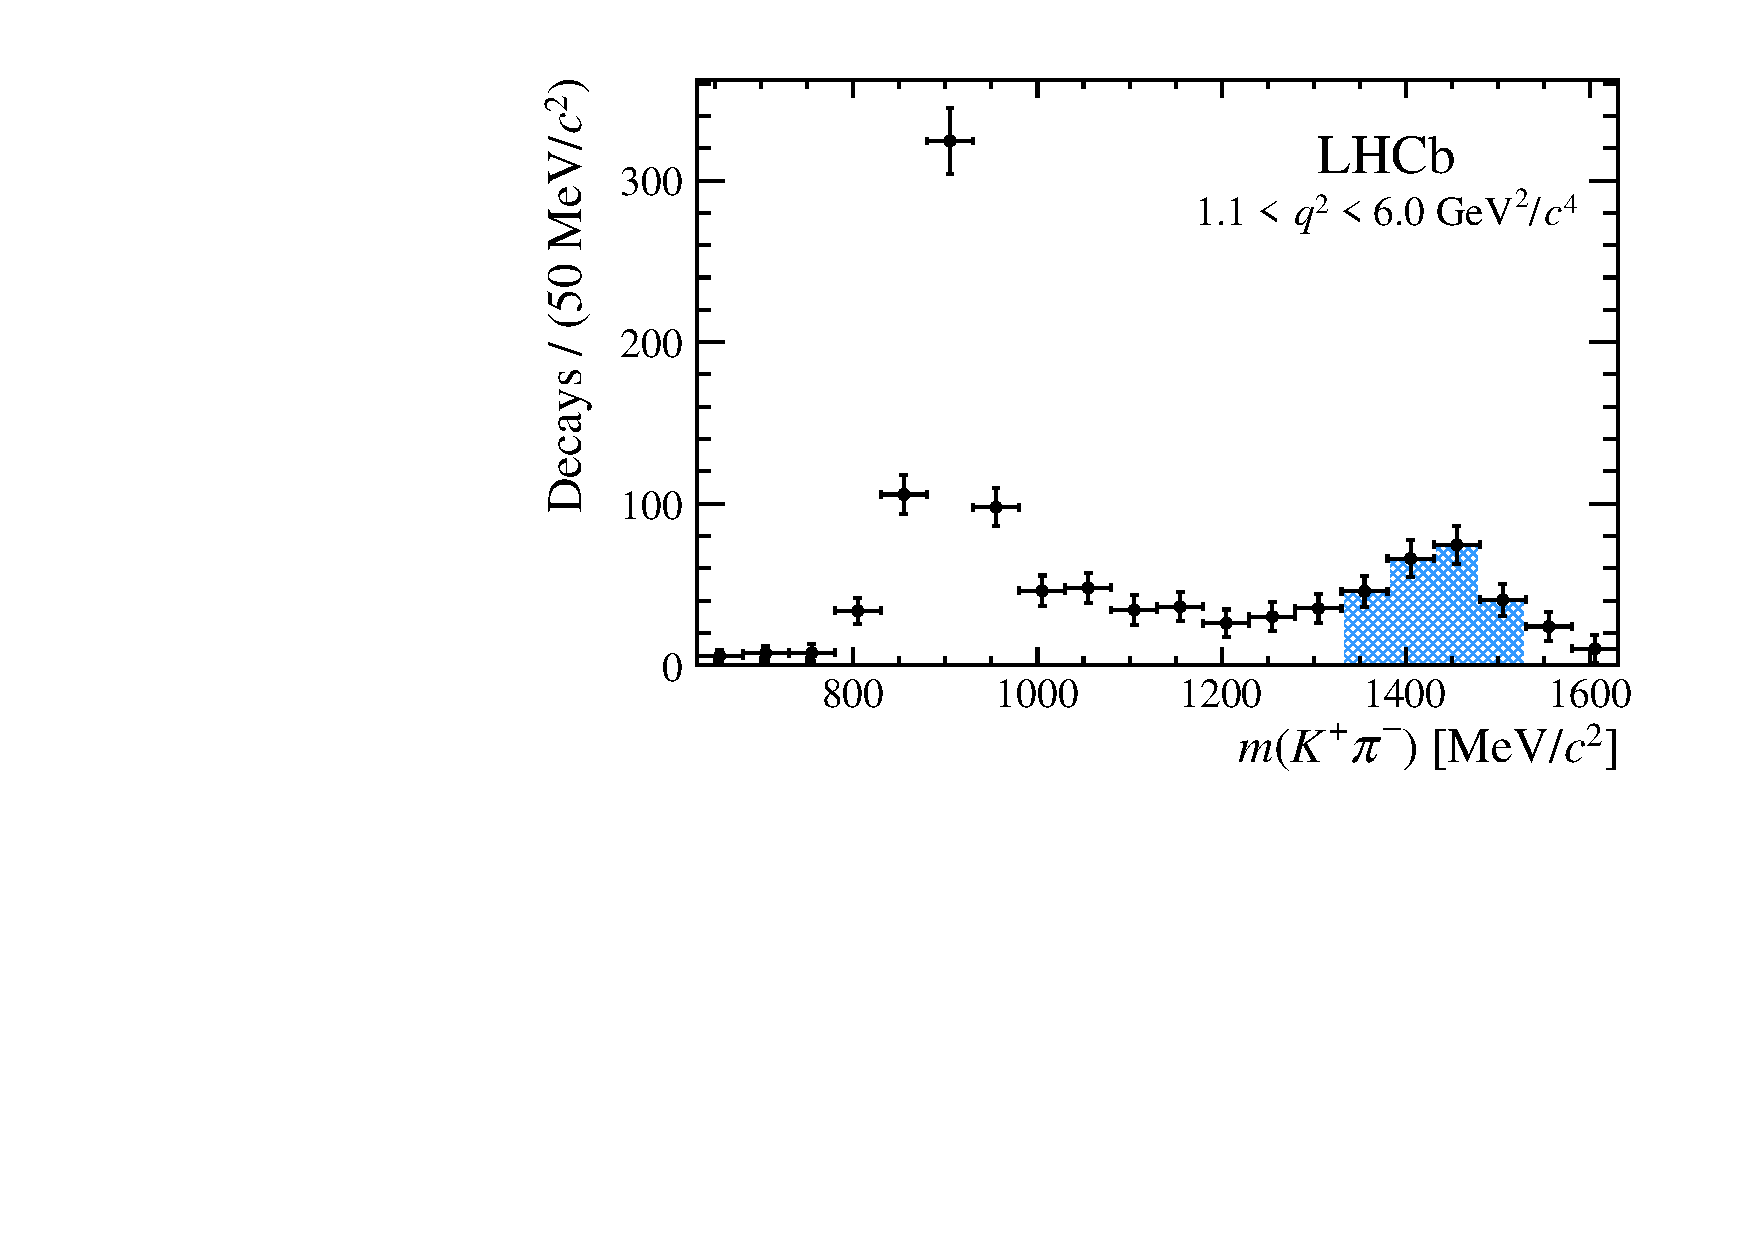
\includegraphics[width=0.6\linewidth]{figs/kpimm/introduction//full-mkpi.pdf}
 \caption{Background subtracted \mkpi distribution in the range $1.1<\qsq<6.0\gevgevcccc$ and $630<\mkpi<1630\mevcc$. The $1330<\mkpi<1530~\mevcc$ region is indicated by the blue shaded area.}
\label{fig:full-mkpi}
\end{figure}

The current chapter describes the measurement of the differential branching fraction and angular analysis of \BdToKpimm in the $1330<\mkpi<1530\mevcc$ region. The values of the differential branching fraction are reported in five narrow bins of the invariant mass squared of the dimuon system, \qsq, between 0.1 and 8.0\gevgevcccc and in the range $1.1<\qsq<6.0\gevgevcccc$,  where an angular moments analysis is also performed. The measurements use the Run 1 data sample collected by the \lhcb experiment, corresponding to an integrated luminosity of $3.0\invfb$. The data were recorded in $pp$ collisions at centre-of-mass energies of $7$ and $8\tev$ during 2011 and 2012, respectively. 

% The decay \BdToKpimm is a rare, FCNC process that proceeds through electroweak penguin or box diagrams in the SM. In extensions to the SM, new heavy particles can enter the loop and modify observables such as branching fractions and kinematic distributions of the final state particles. 

% The previous analyses of \BdToKpimm performed by the \lhcb collaboration~\cite{kstmm-0.3fb,kstmm-1fb,kstmm-1fb-pprime,kstmm-3fb} have focused on the $796<\mkpi<996~\mevcc$ region where the $\kaon\pion$ comes predominately from the P-wave decay $\decay{\Kstarone(892)}{K\pi}$. In this region, the differential branching fraction has been measured along with several different sets of angular observables.

% While the observables measured in~\cite{kstmm-0.3fb,kstmm-1fb} were largely in agreement with SM predictions, a 3.7$\sigma$ local deviation was seen in the observable $P_{5}^{'}$~\cite{kstmm-1fb-pprime}. This deviation was later confirmed by an updated measurement~\cite{kstmm-3fb}. The two results are shown in Fig.~\ref{fig:kpimm:p5prime}. 

% \begin{figure}[!b]
% \centering
% 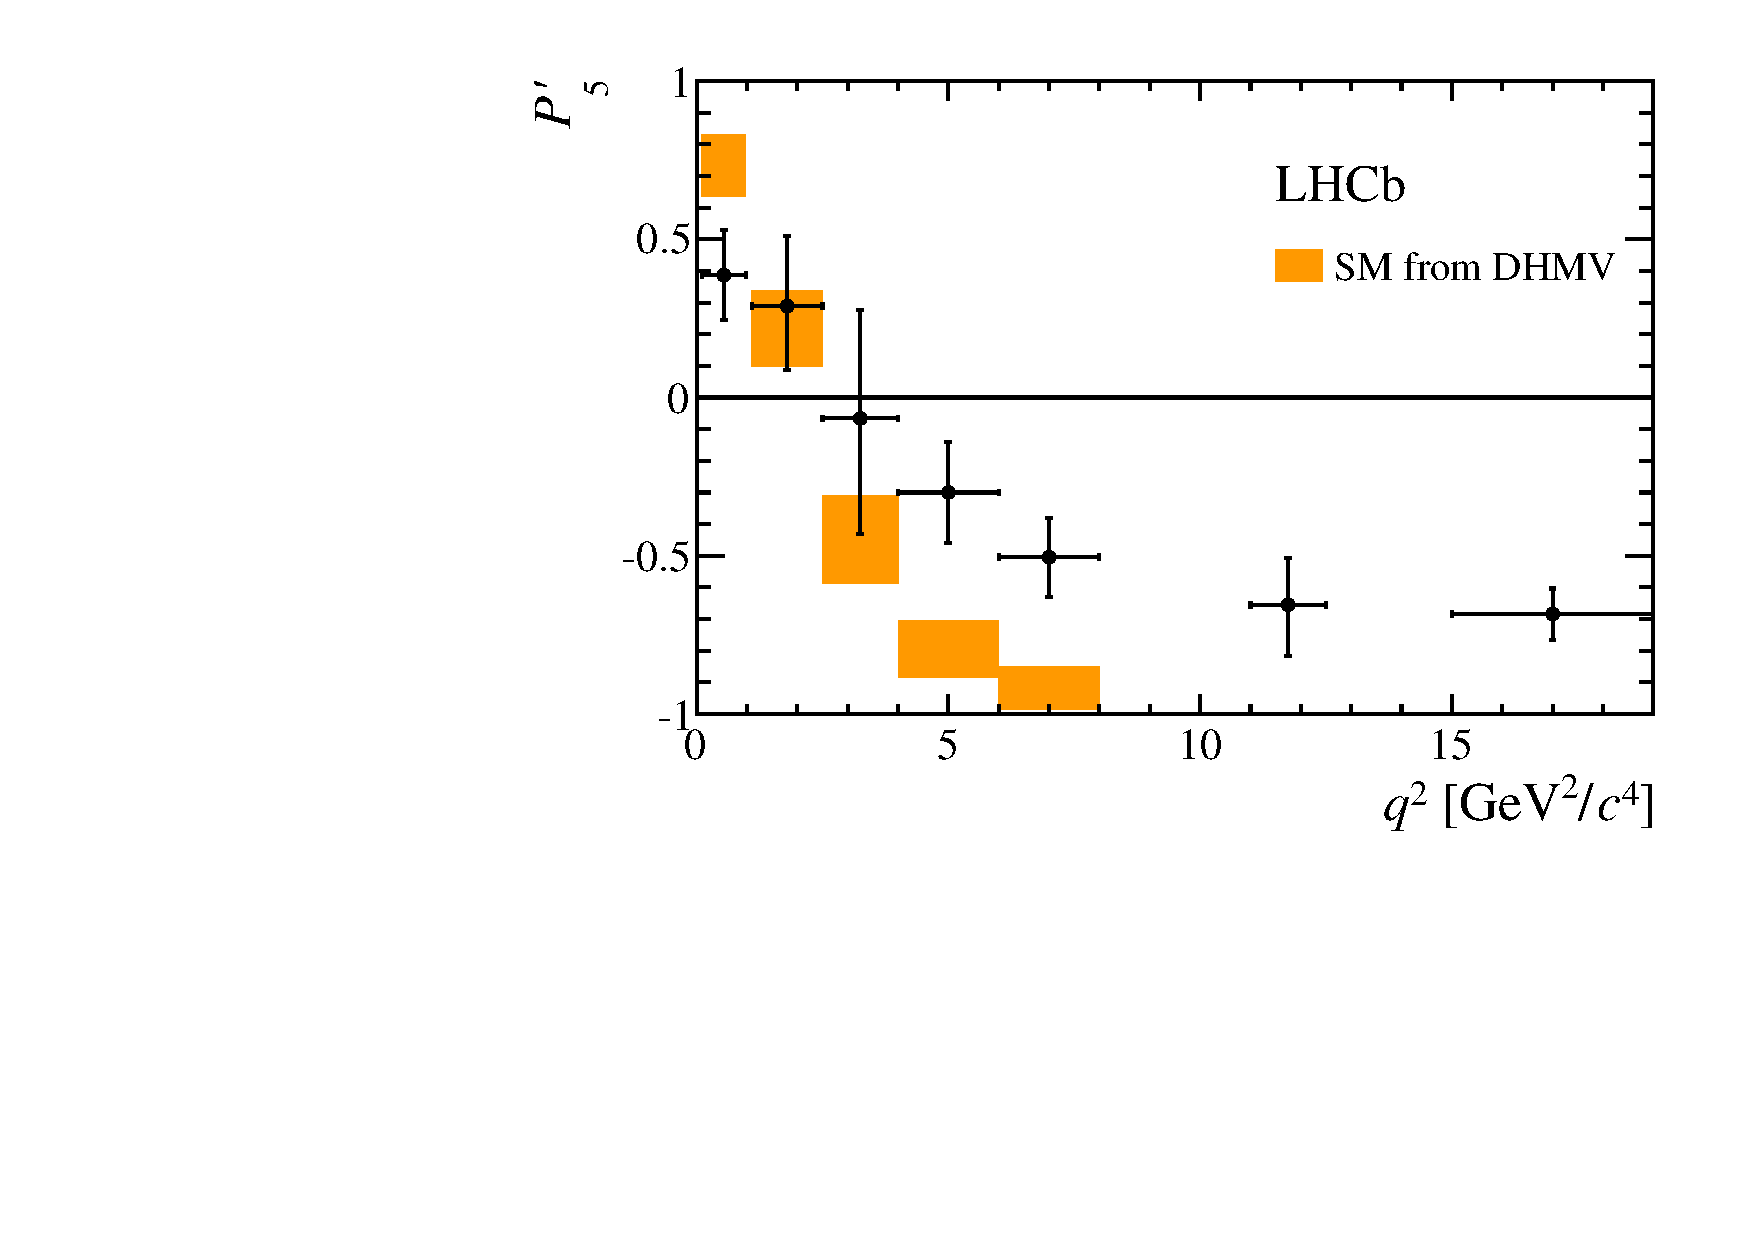
\includegraphics[width=0.8\textwidth]{figs/kpimm/introduction/P5prime.pdf}
% \caption{Results of the measurement of the observable $P_{5}^{'}$ by the \lhcb collaboration. The SM predictions are taken from~\cite{pprime-theory}.}
% \label{fig:kpimm:p5prime}
% \end{figure}

% As shown in Tab.~\ref{tab:introduction:states}, the previously unexplored $1330<\mkpi<1530~\mevcc$ region contains contributions from $S$-, $P$- and $D$-waves. The goal of the following analysis is to measure the differential branching fraction and perform an angular analysis of \BdToKpimm in this \mkpi range.
 
% \begin{table}[!tb]
% \centering
% \caption{Known \KstarJ states that can contribute to \BdToKpimm over the \mkpi range of interest in this analysis. The numerical values are taken from~\cite{pdg}.} 
% \begin{tabular}{c|c|c|c|c}
%    & $J^{P}$ & Mass~[\mevcc] & Full width~[\mevcc]  & $\Gamma_{K\pi}/\Gamma~[\%]$ \\
%   \hline
%   \Kstarone(1410) & $1^{-}$& $1414 \pm 15$& $232 \pm 21$  & 6.6 $\pm$ 1.3 \\
%   \Kstarzero(1430) & $0^{+}$ & $1425 \pm 50$ & $270 \pm 80$ & 93 $\pm$ 10 \\
%   \Kstartwo(1430) & $2^{+}$ & $1432.4\pm 1.3$ & $109 \pm 5$ & 49.9 $\pm$ 1.2 \\
%   %\Kstarone(1680) & $1^{-}$ & $1717 \pm 27$ & $322 \pm 110$ & 38.7 $\pm$ 2.5 \\
%   %\Kstarthree(1780) & $3^{-}$ & $1776 \pm 7$ & $159 \pm 21$ & 18.8 $\pm$ 1.0 \\
%   %\Kstarfour(2045) & $4^{+}$ & $2045 \pm 9$ & $198 \pm 30$ & 9.9 $\pm$ 1.2 \\
% \end{tabular}
% \label{tab:introduction:states}
% \end{table}